\section{Reasoning Guidance through Routing Interventions}
\label{sec:method}

\subsection{Reasoning states and native expert selections}

We relate the visible function of a reasoning sentence to the experts selected by an MoE LLM while its tokens are processed.
%
The state vocabulary $\mathcal C$ contains Read, Analyze, Explore, Plan, Implement, Verify, and Monitor.
%
Read concerns the problem statement, Analyze interprets its constraints, Explore considers alternatives, and Plan organizes subsequent work.
%
Implement carries out a proposed calculation or construction, Verify checks a result, and Monitor assesses progress or the need to revise the approach.
%
The annotation instrument assigns these labels to generated text.
%
They provide observed targets for our analysis.
%

Let $y_s$ denote the assigned class of sentence $s$, and let $T_s$ be its token positions.
%
At routed layer $\ell$ and token $t$, the native selector executes the expert set $S_{\ell,t}$ of size $k_\ell$.
%
An expert identity includes model, layer, and local expert index.
%
For an observed token window $W$, its inclusion frequency is
\begin{equation}
 f_{\ell e}(W)=\frac{1}{|W|}\sum_{t\in W}
 \mathbf{1}\{e\in S_{\ell,t}\}.
 \label{eq:inclusion}
\end{equation}
Each inclusion frequency is between zero and one, and the frequencies sum to $k_\ell$.
%
Dividing them by $k_\ell$ yields a selected-slot distribution over experts.
%
This representation differs from the weights used to combine expert outputs, which may reflect normalization, learned scaling, or a shared-expert path.
%

The architecture's own selection rule defines the native routes.
%
Softmax and sigmoid scores, correction biases, grouped selection, and shared experts can all affect which identities are selected or how their outputs contribute.
%
We therefore compare information and coverage within a model before comparing the resulting summaries across models.
%
We do not align expert indices across models.
%

\subsection{Conditioning routing on a desired reasoning state}
\label{sec:conditioning}

We study expert inclusion and exclusion as interventions on the allocation made by the router.
%
A target set $K_{\ell,c}$ contains $n$ layer-local experts nominated for a reasoning activity $c$ on the training families of the evaluation fold.
%
Nomination ranks experts by their inclusion excess for class $c$ over the other classes, and each class and fold uses the single layer whose nominated set has the largest training association, with stability across training subsamples breaking ties.
%
Activity association alone does not certify that the targets cause it.
%

Let $h_{\ell,t}$ be the layer input at token position $t$, and let $R_\ell$ denote the native router's affinity computation.
%
We write the affinities, the selection priorities, and the native top-$k_\ell$ selection as
\begin{equation}
 q_{\ell,t}=\phi\big(R_\ell(h_{\ell,t})\big),\qquad
 \pi_{\ell,t}=q_{\ell,t}+b_\ell,\qquad
 S_{\ell,t}=\operatorname{top}_{k_\ell}(\pi_{\ell,t}),
 \label{eq:routing-scores}
\end{equation}
where $\phi$ is the model's softmax or sigmoid scoring and $b_\ell$ its selection-correction bias, zero when the router has none.
%
At a frozen prefix ending immediately before $t_0$, the pulse $g_t=\mathbf{1}\{t_0\leq t<t_0+P\}$ covers the states that predict the first $P$ generated tokens.
%
During the pulse, activation and deactivation replace the selected identities by
\begin{equation}
 \widetilde S^{+}_{\ell,t}=K_{\ell,c}\cup\operatorname{top}_{k_\ell-n}\big(\pi_{\ell,t}\big|_{\mathcal E\setminus K_{\ell,c}}\big),\qquad
 \widetilde S^{-}_{\ell,t}=\operatorname{top}_{k_\ell}\big(\pi_{\ell,t}\big|_{\mathcal E\setminus K_{\ell,c}}\big),
 \label{eq:conditioning}
\end{equation}
where $\mathcal E$ is the set of experts at layer $\ell$.
%
The combination weights of the new selection are the native affinities $q_{\ell,t}$ of its members, renormalized and scaled exactly as the native router does.
%
Outside the pulse, at other layers, and after reasoning closes, routing is native.
%
The edit therefore keeps the selection budget $k_\ell$ and the expert-combination rule, and it changes only which experts compute the pulse tokens.
%

\begin{figure}[tb]
\centering
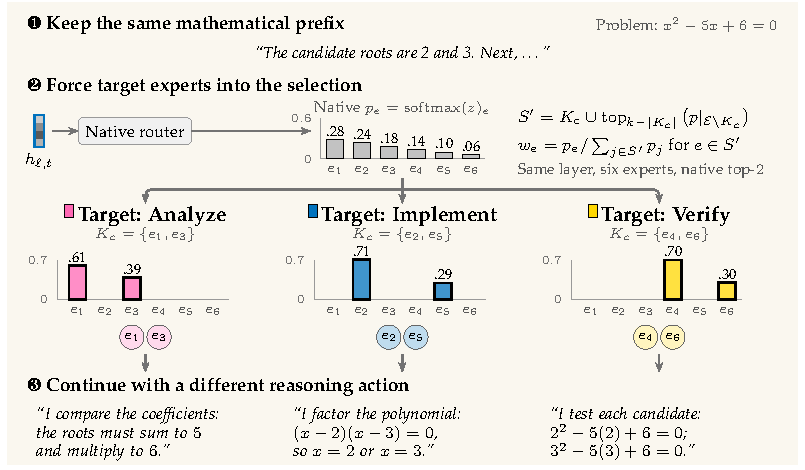
\includegraphics[width=\linewidth]{figures/journal/conditioning.pdf}
\caption{Three class-characteristic continuations from one mathematical prefix.
%
In this constructed softmax example, activation places the indicated expert pair in the top-2 selection and renormalizes their native probabilities.
%
Colored bars and circled IDs identify the top-2 experts.
%
The Analyze, Implement, and Verify continuations illustrate the intervention hypothesis, not measured semantic control.
%
The selection budget and expert-combination rule are retained.}
\label{fig:conditioning}
\end{figure}

The intervention size is the central count $n=\lceil k_\ell/2\rceil$, and the pulse length $P$ is the training median sentence length in tokens.
%
A matched random control replaces $K_{\ell,c}$ by $n$ experts of the same layer drawn from the same native-frequency quintiles and disjoint from every nominated set.
%
Each prefix receives one native continuation and, for every class, targeted activation, targeted deactivation, and the two matched random controls.
%
Comparing a targeted arm with its matched control tests the nominated identities, and comparing either arm with native routing tests the edit itself.
%
All arms of one prefix use the same sampler and seed, and every continuation runs to its natural end or to the original generation allowance.
%
The reasoning state after the edit is read from the first complete sentence and from class occupancy over the next $16\,Q_{75}$ tokens, where $Q_{75}$ is the training upper-quartile sentence length.
%
A lexical classifier trained on the judge-labelled native sentences of the other folds assigns these classes, so no intervention output is relabelled by the judge (Appendix~\ref{app:lexical-readout}).
%
Efficiency is measured by the generated tokens to a final answer and by strict answer accuracy.
%

\subsection{Steering expert selection throughout reasoning}
\label{sec:whole-steering}

A pulse tests whether a local edit redirects the next sentence.
%
Expert steering in MoE LLMs instead fixes expert participation over the whole generation~\citep{fayyaz2025steermoe}.
%
We therefore also steer expert selection at every prompt and reasoning token, from the first prompt token until the reasoning closes, and leave the final answer to native routing.
%

Whole-reasoning steering promotes or suppresses a reasoning activity $c$ through a set $A_c$ of activated and a set $D_c$ of deactivated layer--expert pairs.
%
Nomination uses the inclusion risk difference $\Delta_{\ell,e,c}$, the rate at which expert $e$ of layer $\ell$ is selected on sentences of class $c$ minus its rate on sentences of the other classes, estimated on the training families of each fold and retained only when its sign is stable across subsample refits.
%
Promoting $c$ activates the pairs with the largest positive differences and deactivates those with the most negative ones, whereas suppressing $c$ deactivates the pairs with the largest positive differences.
%
Nominations range over all MoE layers, so a single edit can change many layers at once.
%

At a steered position, the override follows SteerMoE~\citep{fayyaz2025steermoe}.
%
For a softmax router with log-probabilities $s_{\ell,t}=\log q_{\ell,t}$, an activated expert receives $\max_e s_{\ell,t,e}+\epsilon$ and a deactivated expert $\min_e s_{\ell,t,e}-\epsilon$ before the native top-$k_\ell$ selection and renormalization.
%
For a sigmoid router with selection biases, an activated expert takes the affinity $\sigma(\max_e z_{\ell,t,e}+\epsilon)$ of the largest router logit $z_{\ell,t}$ and is always selected, a deactivated expert is never selected, and the combination weights are renormalized and scaled as natively.
%
We use $\epsilon=0.01$, and every layer activates fewer than $k_\ell$ experts and keeps at least $k_\ell$ selectable ones, so the selection budget of Equation~\eqref{eq:routing-scores} is preserved.
%

The edit size follows the counts published for SteerMoE~\citep{fayyaz2025steermoe}.
%
GPT-OSS-20B promotes with 10 activated and 50 deactivated pairs and suppresses with 20 deactivated pairs, and the Qwen models promote with 15 activated pairs and suppress with 500 deactivated pairs.
%
Each other model receives the same share of its own pairs, scaling activation counts by its number of MoE layers and deactivation counts by its number of layer--expert pairs, relative to the 48 layers and 128 experts of Qwen3-30B-A3B.
%
Full, half and quarter strength edit $\lceil f\,n\rceil$ pairs for $f\in\{1,\tfrac12,\tfrac14\}$ and each published count $n$.
%

The direction of each edit comes from the native association between reasoning states and the remaining solution length (Appendix~\ref{app:efficiency-link}).
%
Classes whose sentences precede shorter remaining reasoning at the same question and position are promoted, and classes that precede longer remaining reasoning are suppressed.
%
Each model uses its own pre-registered association, except LFM2.5, whose native association was not part of the pre-registration and which therefore uses the signs pooled across the other models.
%
A matched random control edits the same number of pairs at the same layers, with the same role and from the same native-frequency quintiles, disjoint from the target and from the nominations of the opposite direction.
%
A targeted-minus-random contrast therefore tests the nominated identities at a fixed edit size and placement.
%

Efficiency is the reduction in $\log(1+T)$, where $T$ counts the tokens until the reasoning closes, together with the change in strict accuracy.
%
Steering is efficient when the simultaneous lower bound of the token reduction exceeds zero and the accuracy change stays above $-5$ percentage points.
%
The lexical readout of Appendix~\ref{app:lexical-readout} also measures the share of reasoning tokens in each state, testing whether a promoted state grows and a suppressed state shrinks.
%

\subsection{Incremental information about the present state}
\label{sec:present-method}

The present-state task predicts $y_s$ from the same text context available to the annotation reader.
%
Its baseline representation $x_s$ includes the available previous, current, and next sentences, token identity, position, and sentence length.
%
The routing-augmented representation additionally includes $r_s$, a summary of the sentence's expert allocations.
%
Both classifiers use the same outer evaluation families and the same label targets.
%

Let $a_{\ell,t}$ denote the top-1 expert at layer $\ell$ and token $t$.
%
The sentence histogram and assembled routing vector are
\begin{equation}
\begin{aligned}
 h^{(1)}_{s,\ell e}&=\frac{1}{|T_s|}\sum_{t\in T_s}
 \mathbf{1}\{a_{\ell,t}=e\},\\
 r_s&=Z_{\mathcal T}\!\left(
 D_s\mathbin{\Vert}R_s\mathbin{\Vert}
 P_{\mathcal T}(h^{(1)}_s-\mu_{\mathcal T})\right).
\end{aligned}
\label{eq:present-features}
\end{equation}
Here $\Vert$ concatenates features.
%
The histogram is flattened across layers and experts.
%
Its training mean $\mu_{\mathcal T}$ and principal component projection $P_{\mathcal T}$ are fitted within the training fold.
%
$D_s$ measures depth-path surprise and $R_s$ temporal persistence.
%
$Z_{\mathcal T}$ standardizes each coordinate using that fold's mean and standard deviation.
%
Appendix~\ref{app:readout-features} defines these components and the retained numerical settings.
%

The multinomial ridge readout assigns class probabilities to $v_s$ as
\begin{equation}
 p_{B,b}(c\mid v_s)=
 \frac{\exp(B_{\cdot c}^{\top}v_s+b_c)}
 {\sum_{j\in\mathcal C}\exp(B_{\cdot j}^{\top}v_s+b_j)}.
 \label{eq:readout-map}
\end{equation}
Here $B$ contains one coefficient column per class and $b$ is the intercept vector.
%
For either $v_s=x_s$ or $v_s=[x_s;r_s]$, the fitted parameters minimize
\begin{equation}
 (\widehat B,\widehat b)=\operatorname*{arg\,min}_{B,b}
 \left\{-\frac{\sum_{s\in\mathcal T}w_s\log p_{B,b}(y_s\mid v_s)}
 {\sum_{s\in\mathcal T}w_s}
 +\frac{\lambda}{2}\|B\|_F^2\right\}.
 \label{eq:readout-fit}
\end{equation}
The training sentences $\mathcal T$ receive weights $w_s$ that give each question equal total weight.
%
The penalty leaves the intercept unpenalized.
%
Separate fits for the two inputs give the held-out probability vectors
\begin{equation}
 \begin{aligned}
 \widehat p_x(s)&=
 \bigl(p_{\widehat B_x,\widehat b_x}(c\mid x_s)\bigr)_{c\in\mathcal C},\\
 \widehat p_{x,r}(s)&=
 \bigl(p_{\widehat B_{x,r},\widehat b_{x,r}}(c\mid[x_s;r_s])\bigr)_{c\in\mathcal C}.
 \end{aligned}
 \label{eq:present-predictions}
\end{equation}
All feature transforms and parameter estimates use the corresponding training fold.
%
Setup gives the regularization-selection procedure.
%

We name the held-out reduction in cross-entropy \emph{routing information gain} (RIG).
%
This diagnostic measures how much routing adds to the text baseline when identifying the present state.
%
For text predictions $\widehat p_x$ and routing-augmented predictions $\widehat p_{x,r}$,
\begin{equation}
 \mathrm{RIG}
 =\mathcal L(\widehat p_x,y)-\mathcal L(\widehat p_{x,r},y).
 \label{eq:readout}
\end{equation}
RIG is measured in nats per sentence and can take either sign, with no finite universal bound.
%
Positive RIG supports incremental state information.
%
Loss first averages labelled sentences within a question, then questions receive equal total weight.
%
All training, tuning, and test splits keep duplicate families together.
%

A lexical null preserves the token identities and absolute-position strata used by the control while permuting routing paths within those strata.
%
Repeating the same readout procedure with these paths tests whether the gain depends on the original alignment between routing and reasoning labels.
%
The alignment gain subtracts the observed routing-augmented loss from the mean lexical-null loss.
%
It is measured in nats per sentence and is unbounded in either direction.
%
Positive values support information carried by the original routing alignment.
%
This is a retrospective label-information test because the current and following sentence text are available to the baseline.
%

\subsection{Prediction before the destination sentence}
\label{sec:next-method}

Next-state prediction uses routing from the source sentence to predict the class of its originally adjacent destination.
%
The baseline observes previous and source-sentence text, lexical controls and earlier class history, together with a training-only estimate of the current class.
%
Let $u_s$ collect these baseline features.
%

For this task, $W_s$ contains the last $\min(16,|T_s|)$ owned tokens of the source sentence.
%
Its selected-slot histogram is $h^{(16)}_{s,\ell e}=f_{\ell e}(W_s)/k_\ell$.
%
Training sentences define a marginal routing profile $\pi^0$ and a profile $\pi^c$ for each reasoning class $c$, as detailed in Appendix~\ref{app:next-state}.
%
Their log ratios give seven routing scores and the next-state feature vector
\begin{equation}
\begin{aligned}
 d_{s,c}&=\frac{1}{L}\sum_{\ell=1}^{L}\sum_e
 h^{(16)}_{s,\ell e}\log\frac{\pi^0_{\ell e}}{\pi^c_{\ell e}},\\
 r_s^{\mathrm{next}}&=Z_{\mathcal T}\!\left((d_{s,c})_{c\in\mathcal C}\right).
\end{aligned}
\label{eq:next-features}
\end{equation}
Here $L$ is the number of routed layers.
%
The profiles and coordinate standardization use only the corresponding training fold.
%
Each raw score is a convex average of finite log ratios and can have either sign.
%
For fixed profiles, its bounds are
\begin{equation}
 \frac{1}{L}\sum_{\ell}\min_e\log\frac{\pi^0_{\ell e}}{\pi^c_{\ell e}}
 \;\leq d_{s,c}\leq\;
 \frac{1}{L}\sum_{\ell}\max_e\log\frac{\pi^0_{\ell e}}{\pi^c_{\ell e}}.
\end{equation}
Coordinate standardization subsequently centers and rescales these scores.
%
They summarize all selected slots, separately from the present-state top-1 representation.
%
Both $u_s$ and $r_s^{\mathrm{next}}$ are available before the destination sentence begins.
%
The same multinomial ridge map is fitted separately to $u_s$ and $[u_s;r_s^{\mathrm{next}}]$, using $y_{s+1}$ as the training target and equal total weight per question.
%
Its held-out predictions are
\begin{equation}
 \begin{aligned}
 \widehat p_{\mathrm{past}}(s)&=
 \bigl(p_{\widehat B_{\mathrm{past}},\widehat b_{\mathrm{past}}}(c\mid u_s)\bigr)_{c\in\mathcal C},\\
 \widehat p_{\mathrm{past},r}(s)&=
 \bigl(p_{\widehat B_{\mathrm{past},r},\widehat b_{\mathrm{past},r}}
 (c\mid[u_s;r_s^{\mathrm{next}}])\bigr)_{c\in\mathcal C}.
 \end{aligned}
 \label{eq:next-predictions}
\end{equation}
The current-class estimate itself uses grouped out-of-fold predictions within the training population.
%
The reported losses average held-out log losses across the original repeated fold assignments.
%
The \emph{anticipatory routing gain} (ARG) for the next assigned label is
\begin{equation}
 \mathrm{ARG}=\mathcal L(\widehat p_{\mathrm{past}},y_{s+1})
 -\mathcal L(\widehat p_{\mathrm{past},r},y_{s+1}).
 \label{eq:anticipation}
\end{equation}
ARG is measured in nats per adjacent pair.
%
Positive values support information about a state before its sentence begins.
%
Its range is unbounded in either direction, as for RIG.
%
These names identify the claim and information set of each diagnostic, while both retain the original held-out log-loss estimator.
%

Original sentence indices and reasoning segments determine adjacency.
%
A missing label or a sentence gap breaks the sequence.
%
We retain these breaks instead of connecting the nearest available labels.
%
A source-length sensitivity retains sentences with at least 32 tokens.
%
The routing window already stays inside its source sentence in both conditions.
%
The restriction ensures a full 16-token window and changes the supported population.
%
Present-state and next-state prediction consequently have different information sets and different support.
%

\subsection{Class-balanced expert retention}
\label{sec:selection-method}

The allocation analysis learns a keep-set $K_\ell$ from training families and measures how well it contains held-out native selections.
%
All candidate experts belong to the model's layer-local pool.
%
The methods share the same identity budget $b_\ell$, the same layer and group quotas, and the same training data.
%
Expert ranking uses labelled allocation counts without correctness information.
%

For training family $f$, class $c$, layer $\ell$, and expert $e$, let $C_{fc\ell e}$ be the selected-slot count averaged over the family's member questions.
%
Class balancing normalizes within family and class, averages supported families, then weights classes equally:
\begin{equation}
 s^{\mathrm{bal}}_{\ell e}
 =\frac{1}{|\mathcal C|}\sum_{c\in\mathcal C}
 \frac{1}{|\mathcal F_c|}\sum_{f\in\mathcal F_c}
 \frac{C_{fc\ell e}}{\sum_jC_{fc\ell j}}.
 \label{eq:balanced-selection}
\end{equation}
Here $\mathcal F_c$ contains training families with observed class $c$.
%
Every class must have training support.
%
The normalized scores lie between zero and one.
%
This estimator gives a class equal weight regardless of how much labelled token mass it contributes.
%

The frequency control pools the same labelled counts:
\begin{equation}
 s^{\mathrm{freq}}_{\ell e}
 =\frac{\sum_{f,c}C_{fc\ell e}}{\sum_{f,c,j}C_{fc\ell j}}.
 \label{eq:frequency-selection}
\end{equation}
The methods rank experts by their corresponding training score, apply the common quotas, and break ties by original expert ID.
%
A fixed random selector supplies a third allocation control.
%
Its priorities are independent of the class counts and remain fixed during the comparison.
%

For a held-out family, class, and layer, retained coverage is the fraction of its native selected slots whose expert belongs to $K_\ell$.
%
We average family-weighted coverage equally over routed layers for each class.
%
We call the minimum \emph{weakest-state coverage} (WSC):
\begin{equation}
 \mathrm{WSC}(K)=100\min_{c\in\mathcal C}R_c(K).
 \label{eq:min-coverage}
\end{equation}
WSC ranges from 0 to 100\% and measures whether the retained expert budget contains the native selections of every reasoning activity.
%
The paired \emph{coverage gain},
\begin{equation}
 \Delta\mathrm{WSC}=\mathrm{WSC}(K_{\mathrm{bal}})
 -\mathrm{WSC}(K_{\mathrm{freq}}),
 \label{eq:coverage-gain}
\end{equation}
ranges from $-100$ to $100$ percentage points.
%
Positive values support class balancing for the least-covered activity at the same expert budget.
%
The per-class denominator includes observed labelled selections only.
%
The retained-slot fraction measures containment of the original routes.
%
Rerouting after removal can change the generated solution.
%

\subsection{State distributions and temporal summaries}
\label{sec:dynamics-method}

State occupancy describes how the observed labelled tokens are distributed across the seven classes.
%
For an attempt, class $c$ has occupancy equal to its labelled token count divided by the total labelled token count.
%
Label coverage uses total completion tokens as its denominator.
%
Reporting both prevents a heavily sampled state distribution from being read as full-trace annotation.
%

Within an uninterrupted labelled segment, next-class probabilities use only observed adjacent sentence boundaries.
%
Consecutive sentences with the same class form an observed dwell run.
%
Gaps and the start or end of an observed segment censor the run.
%
These measurements describe the available annotated trajectory.
%
For the native distribution summaries, repeats first average within a benchmark--family occurrence, families average within each benchmark, and the benchmarks receive equal weight.
%

Uncertainty follows the original procedure for each study.
%
Family resampling retains within-family dependence, while the conditional distribution of a fixed fitted readout or selected keep-set omits variation from refitting.
%
We report the scope of each simultaneous correction with its result rather than treating separately constructed panels as one joint test.
%
